\documentclass[a4paper]{article}
%\usepackage{fourier}
\usepackage{marvosym}
\usepackage{hyperref,url}
\usepackage{graphicx}
\pagestyle{empty}
\topmargin=10mm
\textwidth16cm
\hoffset-20mm
\textheight26cm
\voffset-30mm
\pagestyle{plain}
\setlength{\parindent}{0pt} 
\setlength{\parskip}{7pt} 
\hypersetup{colorlinks=true}

\newcommand{\forge}{\textsf{GAGA\space}}

\begin{document}

\begin{center}
\noindent
\textbf{\quad The Australian National University
\hspace*{0.13\textwidth}
College of Engineering and Computer Science} \\[4mm]
%\includegraphics[width=9em]{OutlineLogoBlack.jpg}\hspace*{0.08\textwidth}\space\\
\begin{Large}School of Computer Science
\end{Large}
~ \\[4mm]
\textbf{\begin{Large}COMP2100 $\bullet$ COMP2500 $\bullet$ COMP6442\end{Large}}
~ \\[4mm]
\begin{Large}The Course Project 2011\\[5pt]
        \textbf{\forge}\end{Large}
\end{center}

\hrule

\section*{Introduction}
\label{sec:introduction}

\textbf{S}calable \textbf{V}ector \textbf{G}raphics (SVG) is a standard to create and display
vector graphics material based on the XML (e\textbf{X}tendable \textbf{M}ark-up \textbf{L}anguage).
Vector graphics formats have a number advantages over bitmapped formats (like \emph{JPEG}, \emph{PNG},
\emph{GIF}\ldots) --- much smaller file size, image quality is less affected by display resolution,
ease of creation and editing, other technology can be incorporated to provide advanced features
like animation and widget control (Synchronised Media Integration Language, \emph{JavaScript}),
SVG files can be generated programmatically (especially when a symmetry is involved,
for examples see~\cite{svg-wiki-book}).

SVG describes primitive shapes as leaf-type tag elements, whose style and geometrical
properties specified by the attributes (dimensions, transformation directives,
colours, stroke width and colour \emph{etc}). The primitive elements can be grouped 
together as nested elements inside a container; this allows style, position and 
geometrical characteristics of several elements to be manipulated at once. 

Almost all modern web browsers (except for \emph{Internet Explorer}) can render SVG graphics
(but the extent of the standard implementation varies --- \emph{Safari} and \emph{Opera} can reproduce
animation effects, Firefox --- can't, at least in \texttt{3.x}, all can render gradient effects
and translucency \emph{etc}). Modern vector graphics editors (\emph{Adobe Illustrator} and others) 
can export to SVG format. An open-source editor \emph{Inkscape} uses SVG as native format for its files.

Our project in 2011 is to implement a rendering program which can display a document written in a
\emph{reduced} SVG format. We shall use the Java programming language and Java2D packages, 
in particular, to do this.

\section*{Scalable Vector Graphics format} % (fold)
\label{sec:scalable_vector_graphics_format}

We will work with SVG documents which only contains a \emph{sub-set} all SVG-allowed elements:
primitive graphics elements, their groups and most basic transformations. 

\subsection*{Primitive Graphics Elements} % (fold)
\label{sub:primitive_graphics_elements}

The primitive elements include:
\begin{center}
\begin{tabular}{|l|l|}
        \hline
        \textsf{Line} (interval) & 
        \verb!<line x1="0" y1="100" x2="100" y2="0"! \\
         & \verb!      stroke-width="2" stroke="black" />! \\
        \hline
        \textsf{Rectangle} &
        \verb!<rect x="25" y="70" height="30" width="50"! \\
        & \verb!      fill="#ff8888" stroke="black" stroke-width="2"/>! \\
        \hline
        \textsf{Circle} &
        \verb!<circle cx="140" cy="110" r="60" fill="none"!\\
         & \verb!        stroke="#579" stroke-width="30"! \\
        & \verb!        stroke-dasharray="3,5,8,13">! \\
        \hline
        \textsf{Ellipse} &
        \verb!<ellipse cx="80" cy="170" rx="40" ry="30"!\\
        & \verb!         fill="yellow" stroke="orange" stroke-width="25" />! \\
        \hline
        \textsf{Polyline}
        & \verb+<polyline fill="none" stroke="blue" stroke-width="10"+ \\
        & \verb!          points="50,375 150,375 150,325 250,325 250,375! \\
        & \verb!                  350,375 350,250 450,250 450,375 550,375" />!\\
        \hline
        \textsf{Polygon} & 
        \verb!<polygon points="220,100 300,210 170,250"! \\     
        & \verb!         style="fill:#blue;stroke:red;stroke-width:2"/>!\\
        \hline
\end{tabular}
\end{center}

\begin{center}
\begin{tabular}{|l|l|}
        \hline
        \textsf{Path} & 
        \verb!<path d="M 100 200 Q 200,400 300,200"! \\
        &\verb!      fill="none" stroke="blue" />! \\
        &\verb!<path d="M 100 200 L 200,400 300,200"! \\
        &\verb!      fill="none" stroke="red"/>! \\
        \hline
        \textsf{Text} & \verb!<text x="0" y="100" font-size="80" fill="red">! \\
        & \verb!"Choosing a name for a software program is hard..."</text>! \\
        \hline
        \textsf{Image} & \verb!<image xlink:href="nude.jpg"!\\
        & \verb!       height="200" width="100" x="100" y="100"/>! \\
        \hline
\end{tabular}
\end{center}

The \verb!<image>! element is used to insert a bitmapped image stored in a file. It also allows 
to insert an image described in the SVG format, as well. This last feature and
the powerful \verb!<path>! element, make possible the creation of sophisticated and
visually rich graphics.

The tag element attributes include seen above geometrical and style declarations, and  geometrical transformations which are applied to every pixel of the shape:

\begin{center}
\begin{tabular}{|l|l|}
        \hline
        translate every point by a & \verb!<tag transform="translate(-100,-100)" ... />!\\
        number of pixels in x- and y-directions & \\ 
        \hline
        rotate every point on an angle & \verb!<tag transform="rotate(120,219.5,241)".../>!\\
        around a specified point & \\
        \hline
        scale an object by changing coordinates & \verb!<tag transform="scale(1.2)".../>!\\
        of \textbf{every point} by a common factor & \verb!<tag transform="scale(1.2,0.8)".../>!\\
        (can differ for x- and y-directions) & \\
        \hline
\end{tabular}
\end{center}

Several transformations can be applied simultaneously:
\verb!transform="translate(0,100),scale(0.5)"!.

\subsection*{Container Elements} % (fold)
\label{sub:container_elements}

The container elements can be: \textsf{Svg}, \textsf{Group}, \textsf{Use} and 
\textsf{Definition}. \textsf{Svg} occurs only once in a document --- it is the root of the
content tree. \textsf{Group} allows to group several either primitive or container elements 
together, \textsf{Use} results in expansion in its place the element referenced by its \verb!id!
attribute. The element expanded by \textsf{Use} should be defined elsewhere in the document.
% If \verb!<use>! tag also contains \verb!style! or \verb!transform! attributes, their
% directives will be applied to the expanded elements if their corresponding attributes are
% either not set, of set to \verb!"inherit"! value. 
Finally, \textsf{Definition} allows
to introduce a primitive element or a group to use them elsewhere but \emph{without displaying} 
them immediately.
\begin{center}
\begin{tabular}{|l|l|}
        \hline
        \textsf{Svg} & \verb!<svg xmlns="http://www.w3.org/2000/svg"! \\
        & \verb!     xmlns:xlink="http://www.w3.org/1999/xlink"! \\
        & \verb!     id="svg2" height="700" width="850">! \\
        &  \\
        & \verb!<g ...> ....</g>!\\
        & \verb!<circle ...>...</circle>!\\
        & \verb!...!\\
        & \verb!</svg>!\\
        \hline
        \textsf{Group} & \verb!<g transform="translate(120,0)" fill="#bbb">! \\
        &\verb!    <rect x="100" y="100" width="100" height="20" fill="inherit" />! \\
        &\verb!    <ellipse id="e1" cx="150" cy="140" rx="30" ry="100" fill="#707" />! \\
        &\verb!    <rect x="100" y="130" width="100" height="20" fill="inherit" />! \\
        & </g>\\
        \hline
% \end{tabular}
% \end{center}
% 
% \begin{center}
% \begin{tabular}{|l|l|}
%       \hline
        \textsf{Use} & \verb!<g id="G" >! \\
        &\verb!    <rect x="100" y="100" width="100" height="20" fill="inherit" />! \\
        &\verb!    <ellipse id="e1" cx="150" cy="140" rx="30" ry="100" fill="#777" />! \\
        &\verb!    <rect x="100" y="130" width="100" height="20" fill="red" />! \\
        &\verb!</g>!\\
        & \\
        & \verb!<use xlink:href="#G" transform="translate(120,0)" fill="#bbb"/>!\\
        & \verb!<use xlink:href="#e1" transform="scale(1.2)" fill="#777"/>!\\
        \hline
        \textsf{Definition} & \verb!<defs> ... </defs>!\\
        & (defines an element or a group, but does not display it; can be displayed with \verb!<use>!) \\
        \hline
\end{tabular}
\end{center}

The style attributes in elements inside a container, which are unset (defaulted), or set to
\verb!"inherit"! value, will be set to the corresponding values set in the parent container 
element (this works for all container elements --- \verb!<svg>!, \verb!<g>! and \verb!<use>!).

The full SVG specification contains advanced features like gradients, colour filters
(blurring, distortion, \emph{etc}), object morphologies, patterns, masks, region clipping
and so on. Not all of them are currently implemented by applications which were deemed to be
the primary users of the SVG format (namely, web browsers). Among the advanced features are
animations and dynamic effects (like interactive SVG images which contain embedded
control widgets). Some of them are partially implements. In the beginning, we will not use the 
above advanced features of SVG, and will only try to implement primitive graphics objects 
and containers listed above.

\section*{\forge --- a Java SVG Renderer} % (fold)
\label{sec:forge_a_java_svg_renderer}

The beta-version of \forge is capable of parsing an SVG file which contains a description of a
scene graph using the reduced subset of SVG tags; it builds a document tree, performs
its (incomplete) validations, and renders the scene graph using \emph{Java2D} graphics
package. \forge implementation is incomplete. The salient lacking features include:

\begin{enumerate}
        \item The program is yet to be able to process \textsf{Polyline}, \textsf{Polygon} and 
        \textsf{Path} and \textsf{Image} graphics elements.
        \item Colours (for \verb!fill! and \verb!stroke! attributes) can only be described
        in the \verb!octal! or \verb!hexadecimal! formats (\emph{eg}, \verb!fill="#ff0000"! 
        can be processed, but \verb!fill="red"! can't!) 
        \item In its dealing with the element attributes, \forge 
        currently can only understand style directives given in the form of \verb!key="value"!,
        but unable to process style information provided in CSS style (see below).
        \item It cannot process style and transformation defined in group elements and apply them
        to the nested container and graphics elements.
        \item It cannot apply \textsf{Use} expansions because it must first collect all
        elements marked by the \verb!id! attribute, but this feature is not yet implemented.
\end{enumerate}

\vfill

\pagebreak

\section*{The \forge Architecture} % (fold)
\label{sec:the_forge_architecture}

\enlargethispage{1cm}
\forge has a pipe-line architecture: the input character stream is broken into stream of tokens, 
which are then parsed to build the document tree (called here \emph{a scene graph}), which then
can be processed (validated, modified), and finally rendered in an Java graphical application 
window, Figure~\ref{fig:pipeline}.

\begin{center}
\begin{figure}[ht]
% \hspace{0.05\textwidth}
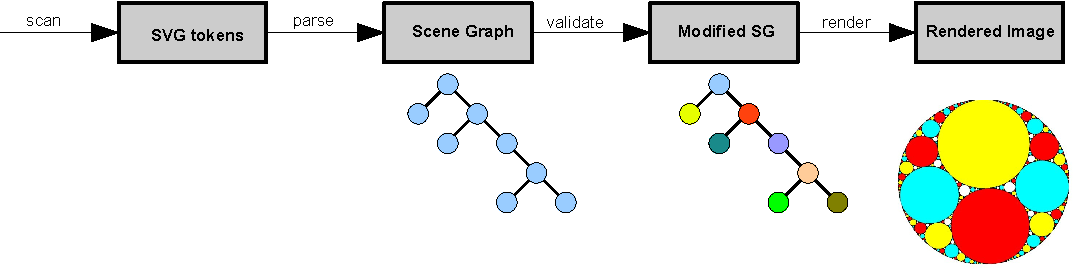
\includegraphics[width=1.0\textwidth]{forge-pipe.pdf} 
\caption{Pipe-line architecture of an XML processing system like \forge}
\label{fig:pipeline}
\end{figure}
\end{center}

The stages in more detail:

\begin{enumerate}
        \item \emph{Scanning} is done using the standard \emph{SAX} (\textbf{S}imple \textbf{A}PI 
        for \textbf{X}ML) API from the Java standard library (the \texttt{org.xml.sax} package). 
        The SAX class \emph{DefaultHandler} is extended to implement the event handlers which
        are called when the scanner processes XML tags:
        \begin{itemize}
                \item \verb!startDocument()! and \verb!endDocument()! to signal the beginning and the
                end of the entire document
                \item \verb!startElement()! and \verb!endElement()! to signal the opening and closing 
                element tags (name and attributes are retrieved as the method parameters)
                \item \verb!characters()! to collect and process characters inside a tag element
        \end{itemize}
        The SAX API also provide event handlers to process comments, processing instructions,
        DTDs, resolve entities and check for errors (for example, whether the document is well formed
        \emph{etc}). We only implement the begin/end event handlers for the tags (and the document)
        and characters assuming that we only deal with well formed SVG documents. We do not make
        use of DTD or PI event handlers since our program itself defines how the tags need to be
        processed and rendered.
        \item We build the parse tree (aka \emph{scene graph}) ourselves without using DTD/Schema
        provided by the \textsf{W3C SVG} specification. The tag parsing and tree building
        are done by the \emph{SvgScanner} class (the one which extends \emph{DefaultHandler}), 
        which maps tag name and attributes into objects of the \emph{SvgElement} hierarchy and creates 
        a parse tree with the structure of the parsed SVG document.
        \item The scene graph is processed by \emph{Visitor} objects, which validate, modify
        and render the scene graph. Rendering is done with \emph{Java2D} graphics library
        (packages \verb!java.awt!, \verb!java.awt.geom!, \verb!java.awt.image! and others).
        \item The structure of the scene graph is defined as the \emph{Composite} pattern,
        and it is shown on the Figure~\ref{fig:composite}.
        \item The \emph{SvgElement} specialisation into different container and graphics elements
        is done via a composition of an element and its \emph{Type} (this solution
        employs the \emph{Strategy} pattern, when the specialisation of types is achieved not 
        through subclassing but through composition with an appropriate object
        from the \emph{Type} hierarchy).
        \item The tree processing and rendering is done by visitor objects
        which are defined in a separate (from the \emph{SvgElement}) hierarchy, formed
        by the \emph{Visitor} interface. The \emph{Visitor} interface matches the concrete
        classes in the \texttt{Element--Type} hierarchy. The concrete \emph{Visitor} objects
        perform element specific operations (like rendering) when called by the corresponding
        element object. The \emph{Visitor} pattern is a well known solution to remove operations
        performed by an object hierarchy outside the hierarchy, and by this to make addition of
        new operations (or change existing ones) independent from the hierarchy itself.
        In greater details the \emph{Visitor} pattern is discussed in the lectures.
\end{enumerate}

\begin{center}
\begin{figure}[ht]
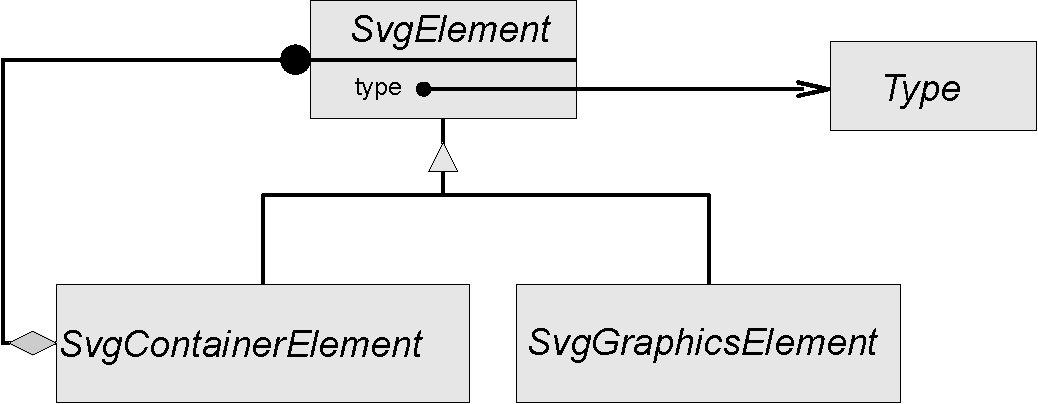
\includegraphics[width=0.45\textwidth]{forge-composite.pdf}\hspace{0.1\textwidth}
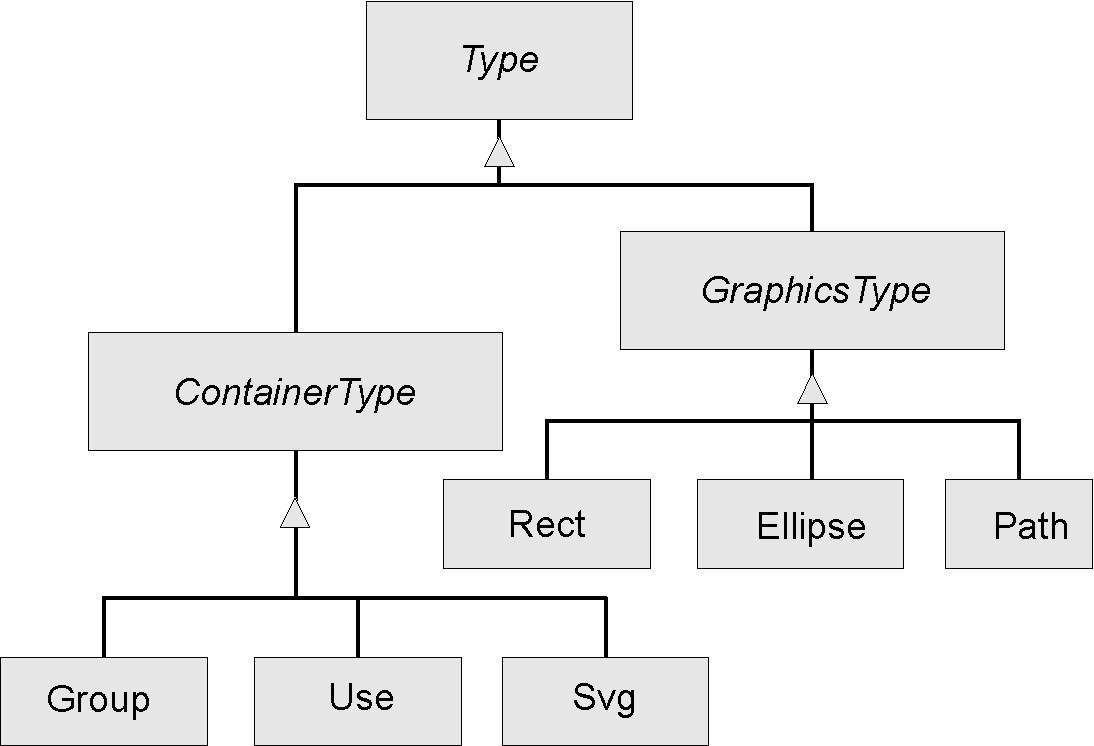
\includegraphics[width=0.45\textwidth]{forge-composite-type.pdf}
\caption{\textbf{Left}: Composite structure of the \emph{SvgElement} hierarchy.
\quad\textbf{Right}: \emph{Type}'s hierarchy.}
\label{fig:composite}
\end{figure}
\end{center}

\section*{Notes on literature and the name ``GAGA''} 
\label{sec:notes}

The project will require additional studies of the XML, SVG and SAX (and the design
patterns used in the original code). The two tutorials, \cite{svg-tutorial-1} and
\cite{svg-tutorial-2}, can be helpful, alongside with the official SVG standard, 
\cite{svg-draft}. If you are not afraid of looking into a large code base, some ideas
about how a rendering system like \forge can be designed and implemented (at a much higher
level of functionality), check out the Apache's \emph{Batik} project, \cite{batik}.
But know this --- the \emph{Batik} design and implementation did not influence the
\forge project in a slightest degree (we wanted to keep things at a more elementary level
\footnote{And we also prefer to write our own code {\large\Smiley}.}).

Why the name ``GAGA''? Honestly, it's not after Lady GAGA, or the song
``Radio Ga-Ga'' (one author is not Lady GAGA's fan, to say the least, and he has long
overgrown \emph{Queen}'s music). ``GAGA'' simply means ``Give Assistance to Graphics Authors'',
which is the testimony to our lame imagination. Full stop.

% The original plan was to write a rendering program to deal with files
% created by the Open-Office drawing suite. The name ``OGRE'' (\textbf{O}pen-Office
% \textbf{G}raphics \textbf{R}endering \textbf{E}xperiment) sounded like a good name. When
% later we decided to use the SVG format, there was no case for the letter `O', but
% ``OGRE'' was already too dear to us to drop it. So, we kept it by qualifying its
% current status --- \forge is ``Formely Open-Office Rendering Graphics Experiment''
% (`G' and `R' had to swap places because, well, ``Fogre'' sounds like ``Focker'', which
% may be a good name for Hollywood, not for us). 


\bigskip
\begin{thebibliography}{999}

\bibitem{svg-tutorial-1} David Dailey, 
\href{http://www.w3.org/Graphics/SVG/IG/resources/svgprimer.html}{``An SVG Primer for Today's Browsers''}
An official tutorial with links to appropriate standard specification
details.//
\href{http://www.w3.org/Graphics/SVG/IG/resources/svgprimer.html}{http://www.w3.org/Graphics/SVG/IG/resources/svgprimer.html}

\bibitem{svg-tutorial-2} Gerald Bauer,
\href{http://luxor-xul.sourceforge.net/talk/jug-nov-2002/slides.html}{``Scalable Vector Graphics (SVG).
Creating High-End 2D Graphics Using XML''} An old but useful SVG
tutorial.\\
\href{http://luxor-xul.sourceforge.net/talk/jug-nov-2002/slides.html}{http://luxor-xul.sourceforge.net/talk/jug-nov-2002/slides.html}

\bibitem{svg-draft} The W3C SVG Standard Draft, \href{http://www.w3.org/TR/SVG11/}{``Scalable 
Vector Graphics (SVG) 1.1 (Second Edition) W3C Working Draft 22 June 2010''} \href{http://www.w3.org/TR/SVG11/}{http://www.w3.org/TR/SVG11/}

\bibitem{batik} \href{http://xmlgraphics.apache.org/batik/}{``\emph{Batik}, An SVG Java Toolkit''},\href{http://xmlgraphics.apache.org/batik/}{http://xmlgraphics.apache.org/batik/}\\
An \emph{Apache} toolkit for applications or applets that want to use images in the Scalable Vector
Graphics. An open source Java framework which implements a large part (but not all!) of the 
SVG specification. The framework is used in an SVG rendered/editor,
\href{http://apache.mirror.aussiehq.net.au/xmlgraphics/batik/Squiggle-1.7.dmg}{\emph{Squiggle}}
(for Mac OS X only).\href{http://apache.mirror.aussiehq.net.au/xmlgraphics/batik/Squiggle-1.7.dmg}{http://apache.mirror.aussiehq.net.au/xmlgraphics/batik/Squiggle-1.7.dmg}

\bibitem{svg-wiki-book}\href{http://en.wikibooks.org/wiki/XML_-_Managing_Data_Exchange/SVG}%
{XML - Managing Data Exchange/SVG}, A Wiki book about SVG.\\


\end{thebibliography}
\vfill
%\hrule

\begin{flushright}
{\fontfamily{pzc}\fontseries{m}\fontshape{it}\fontencoding{T1}%
\fontsize{13pt}{14pt}\selectfont 
School of Computer Science, ANU \\
Chris Johnson, Alexei Khorev \\ 
\today\space }
\end{flushright}

\end{document}
